\newpage

\section*{ $^{24}$Cu(n,p)$^{24}$Na }

Power Level: 100 kW(th) \\
Time at Power: 60.0 m \\
Wait Time:  2.0 d \\
Counting Time: 60.0 m \\
Total Activity at Removal: 4.12e-02 $\mu Ci$

\begin{table*}[h]
\centering
\begin{tabular}{ |c|c|c|c|c|c| }
 \hline
 Position & Mass $mg$ & Counting Activity $\mu Ci$ & Area (Counts) & Error \% \\
 \hline 
 1 & 0.26 & 1.07e-03 & 2.09e+03 & 2.1849 \\ 
\hline
 2 & 0.26 & 1.60e-03 & 3.12e+03 & 1.7892 \\ 
\hline
 3 & 0.26 & 1.23e-03 & 2.40e+03 & 2.0393 \\ 
\hline
 4 & 0.26 & 5.46e-04 & 1.07e+03 & 3.0630 \\ 
\hline
\end{tabular}
\end{table*}

\begin{figure}[h]
\centering
\begin{subfigure}{.5\textwidth}
  \centering
     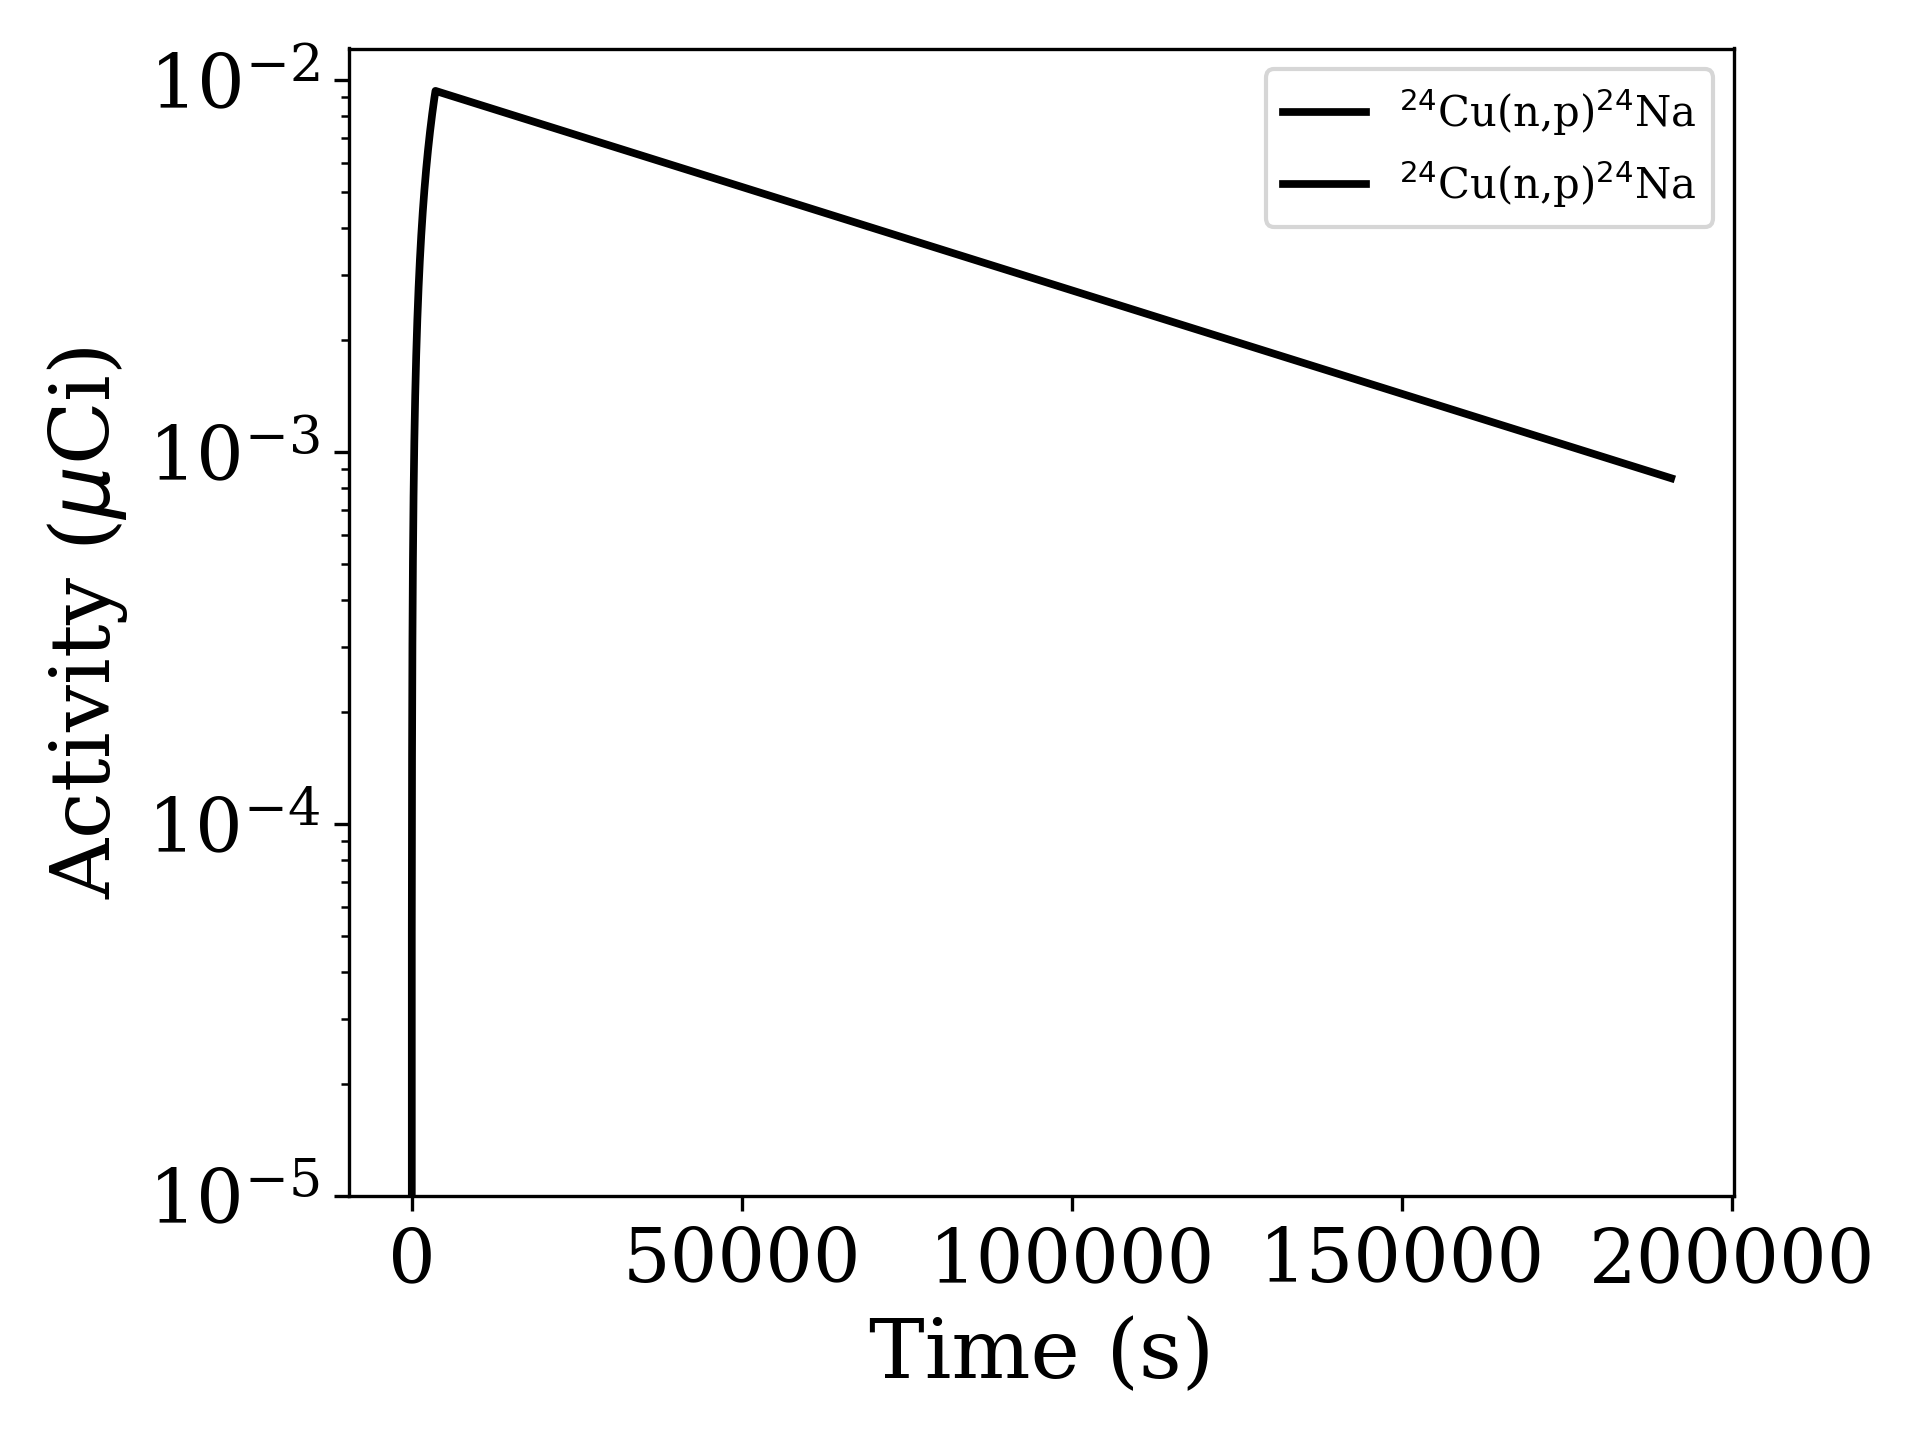
\includegraphics[width=.8\textwidth]{plot/Cu-24(n,p)Na-24_library1} 

  \caption{A subfigure}
  \label{fig:sub1}
\end{subfigure}%
\begin{subfigure}{.5\textwidth}
  \centering
     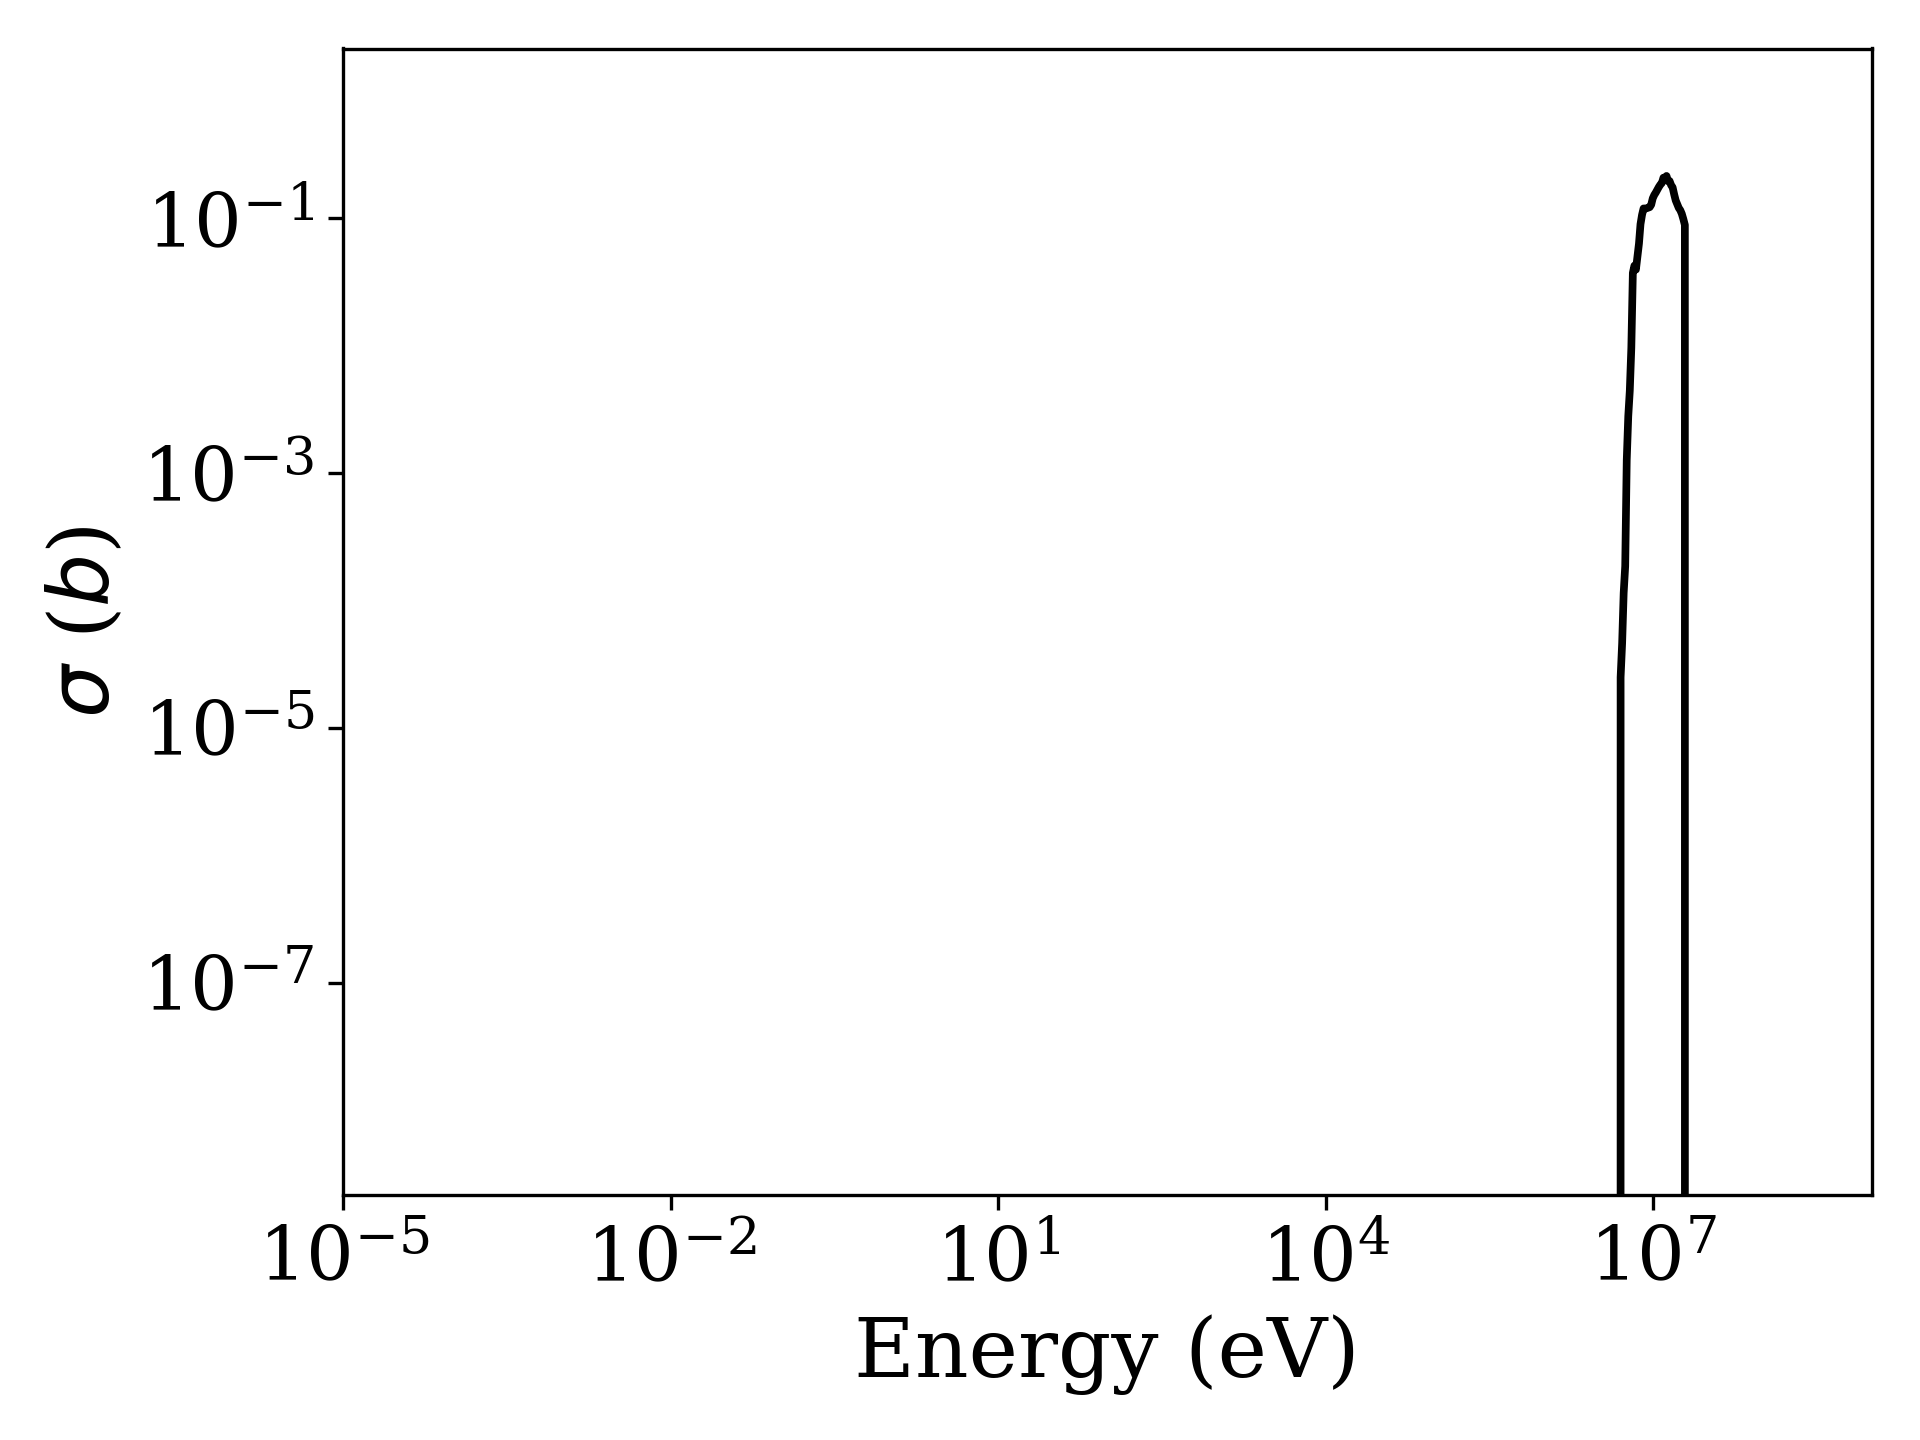
\includegraphics[width=.8\textwidth]{plot/Cu-24(n,p)Na-24} 

  \caption{A subfigure}
  \label{fig:sub2}
\end{subfigure}
\caption{A figure with two subfigures}
\label{fig:test}
\end{figure}

\begin{table*}[h]
\centering
\begin{tabular}{ |c|c|c|c|c|c|c| }
 \hline
 Reaction & T$_{1/2}$ & ROI (eV) & Important Gammas (keV) \\
 \hline 
 $^{24}$Cu(n,p)$^{24}$Na & 15.0 h & 6.46e+06, 1.18e+07 & 1368.626(0.999936) \\ 
\hline
\end{tabular}
\end{table*}
